Under praksisperioden hos Solwr jobbet jeg primært med å bidra til utviklingen av \textit{TRACE Insigh}t, et analyseverktøy for kunder. En av hovedoppgavene var å implementere en modul, som bruker \gls{abc}-analyse. Modulen ble utviklet ved å konvertere en eksisterende Python-applikasjon til en Java-applikasjon og integrere denne i \textit{TRACE Insight}. Backend ble skrevet i Java, frontend i Vue3, og dataen ble hentet fra databasen gjennom \gls{sql}-queryer. \\

Arbeidet startet med å sette opp arbeidsmiljøet, som inkluderte Linux (Ubuntu), \Gls{git}, og \gls{vsc}. Oppgavene omfattet utvikling av \gls{sql}-queryer for å simulere realistiske datauttrekk fra bedriftens database, samt oversettelse av modulen for å støtte både norsk og engelsk gjennom internasjonalisering. \\

Gjennom hele perioden var det tett samarbeid med både veileder og kolleger. Andrea Tenti, min veileder, hjalp med forståelse av matematiske algoritmer og navigasjon i databasen. Andre ansatte, som Halvard Øverlien og Mikael Tollefsen, bidro med teknisk støtte, feilsøking, og anbefalinger om beste praksis for \gls{api}-utvikling. \\

Resultatet av arbeidet var en fungerende Java-basert \gls{abc}-modul som simulerte kostnadsanalyser ved å vise data i ulike visuelle formater, inkludert stolpediagrammer og doughnut-diagrammer. Selv om dataene i modulen var tilfeldig generert, ga applikasjonen en \textit{proof of concept} som virksomheten kunne bygge videre på. \\

Totalt ble 123 timer fullført, med en økning i arbeidsmengde mot slutten av praksisperioden for å sikre at alt ble ferdigstilt før eksamensperioden. Tidsfordelingen ble nøye dokumentert, og arbeidet ble utført ved hjelp av en kombinasjon av selvstendig arbeid og samarbeid i team. \\

Praksisarbeidet la grunnlaget for videre utvikling av modulen, og virksomheten planlegger å videreføre dette arbeidet internt for å gjøre løsningen fullt operativ.

\subsubsection{Log for hver arbeidsdag}
\logg{Torsdag 12. September}{10:00 til 16:00 (6 timer)}{
Møtte opp klokken 09:45 for å delta på oppstartsmøte som skulle starte klokken 10:00. På møtet ble det informert om at alle praksis-studentene skal deles opp inn i forskjellige prosjekter. Deretter blir alle prosjektene presentert; 'research and development', 'digital integration' og 'service and design'.\\

Studentene fikk velge fritt om hvilke av prosjektene de ville delta på. Studenten \textit{Vegard Arnesen Mytting} meldte seg til prosjektet sammen med \textit{Research and Development} avdelingen, sammen med to andre medstudenter. \\

Der får studentene vite at de skal få utdelt arbeids-laptoper, hvor de da skal installere Linux (Ubuntu) som operativsystem. Dette blir startet, og det blir fort oppdaget at dette var utfordrende, ettersom Windows' \textit{Bit Locker} ikke ville tillate Ubuntu. Dette førte oss til å få hjelp av en som jobber på bedriften til å fikse alle laptopene til dem som hadde dette problemet. \\

Etter at Linux ble installert på laptopen, ble det spist lunsj sammen med hele \textit{RnD} gruppen. Der var det brødskiver og en salatbar. \\

Etter lunsjen var det på tide å installere alle programmene man vil trenge til å kunne jobbe. Da måtte man installere \textit{Visual Studio Code}, for å kunne kode og utvikle. \textit{Git} for versjonskontroll og for å kunne hente repositoriet til koden. \textit{Slack} for kommunikasjon mellom gruppen. \textit{Postgresql} for å kunne få tilgang til databasen til prosjektet. \textit{DBeaver} for å kunne bearbeide og arbeide med databasen. \textit{Conda} for å skaffe seg et Python utviklingsmiljø. Til slutt \textit{Docker} for å kunne bygge og teste applikasjonen som skal bli jobbet med.

\begin{figure}[H]
\centering
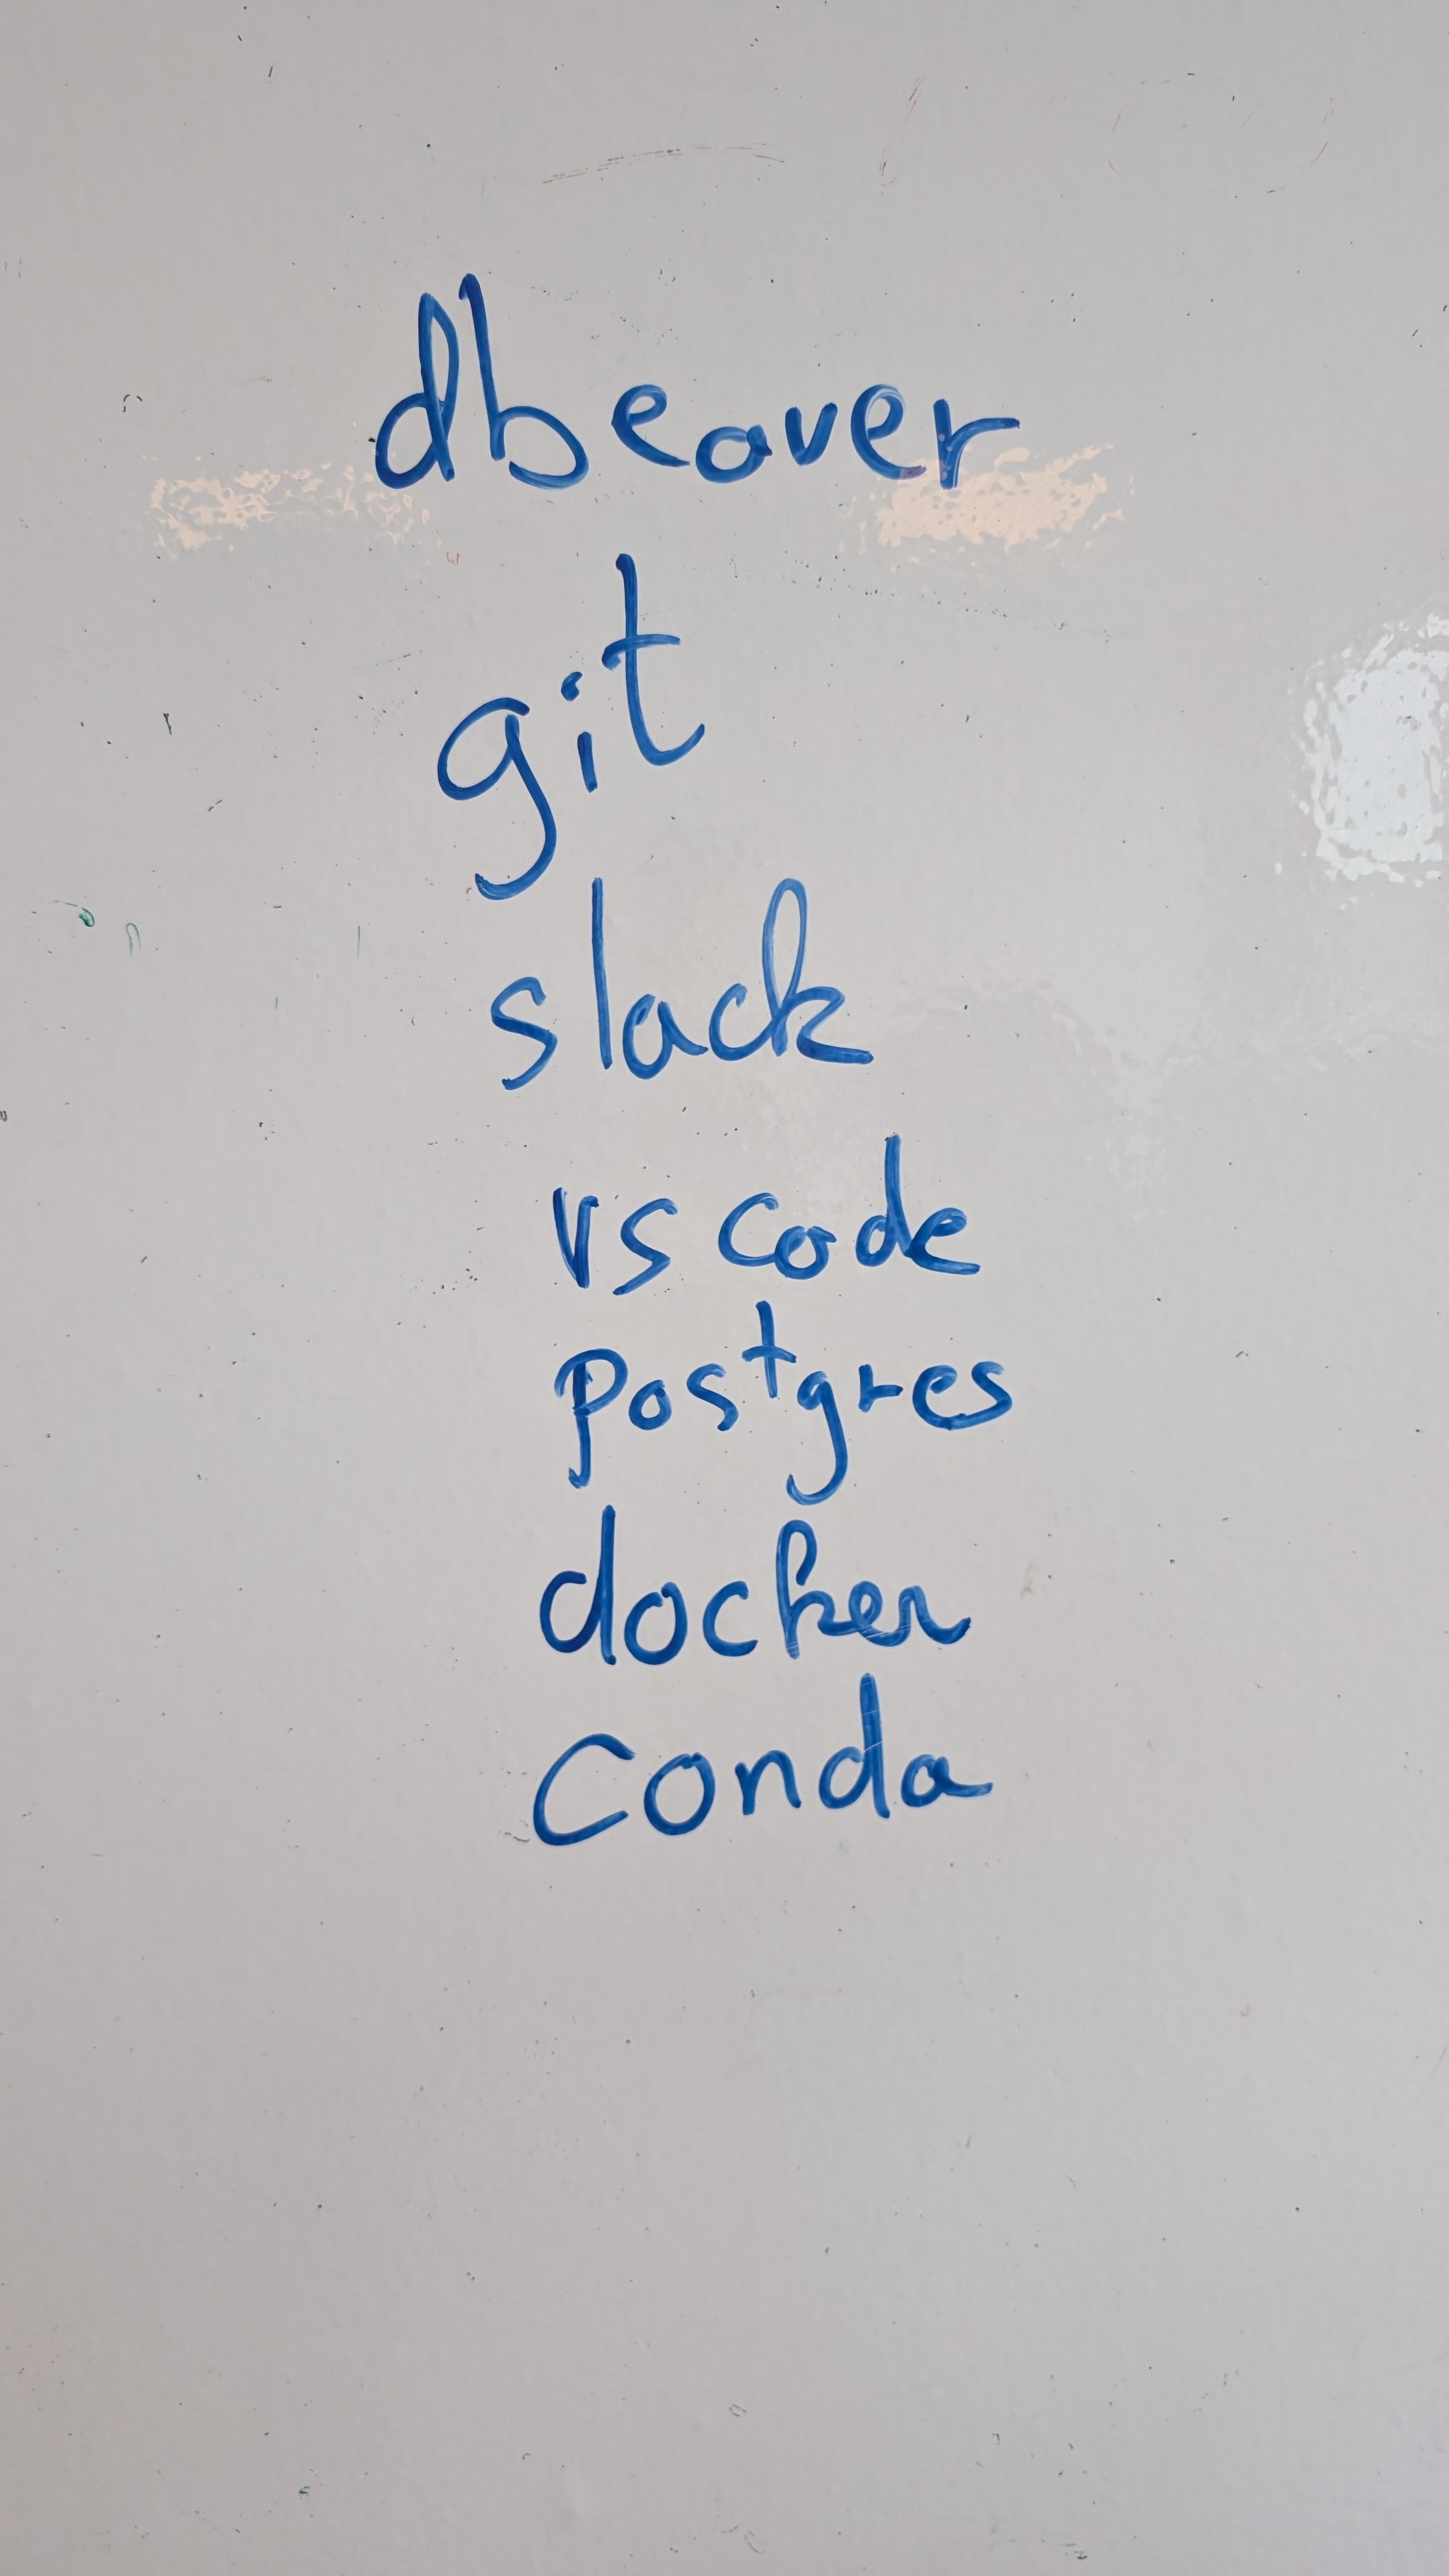
\includegraphics[width=0.25\linewidth]{ukentlige logger/images/uke 1/programs_to_download.jpg}
\caption{\label{fig:downloads}Liste over programmer som skal lastes ned.}
\end{figure}

Det ble noen problemer ved nedlastningen av disse programmene. 

\begin{itemize}
    \item Slack ble lasted ned, men var ikke mulig å åpne. Det ble enig om at studenten skal bruke den nett-baserte versjonen av Slack, dersom det blir behov. 
    \item Visual Studio Code fikk problemer når man skulle begynne å installere \textit{extentions}. Enkelte utvidelser gikk greit, mens andre gjorde det umulig å jobbe i programmet (Programmet kjørte ikke).
\end{itemize}

Etter at alt ble installert var klokken 16:00. Studenten pakket da sammen og dro hjem. 
}\\\\\\
\logg{Onsdag 18. September}{10:00 til 14:00 (4 timer)}{
Møtte opp klokken 10:00 for å fortsette forbredelser til fremtidig arbeid. Her begynte studenten å bygge en postgres database på laptopen som ble utdelt. Der fikk studenten en \textit{dump} fil, hvor det ligger mye data som skal bli brukt i prosjektet. Studenten forsøkte å bygge databasen med hjelp fra DBeaver programmet som ble lastet ned forrige uke, men dette viste seg å være en utfordring. Det endte med at studenten skapte en database ved hjelp av kommandolinjen. Når studenten skulle \textit{restore} dataen fra dump filen, oppstod det noen problemer. Studenten valgte da å gjøre litt research på hva man kan gjøre for å gjenopprette dataen. \\

Etter flere forsøk uten noen framgang, valgte studenten å se mer på \textit{trace-insight} applikasjonen. Her var det den \textit{README.md} fil hvor det var instrukser på hva man må gjøre for å få applikasjonen til å kjøre. Applikasjonen bruker bruker fire teknologier. \textit{Gardle}, \textit{Node}, \textit{Docker}, og \textit{Postgres}. Det var skrevet i dokumentasjonen at man måtte starte starte backend og fortsend for å bruke applikasjonen i localhost. Npr studenten skulle starte backend feilet systemet å bygge den. Studenten prøvde da å starte froentend for å se om den måtte kjøre først. Frontend fungerte, men applikasjonen var helt hvit. Dette var grunnet at hvis backend ikke kjører, skal ingenting vises. Studenten forsøkte da å installere Gradle og forstatte å lese dokumentasjon på denne teknologien for å prøve å finne feilen. \\

Med lite progresjon, bestemte eleven seg for å lese seg opp på \textit{abc-analyse} og dokumentasjon på en annen applikasjon (som fungerte).

\begin{figure}[H]
\centering
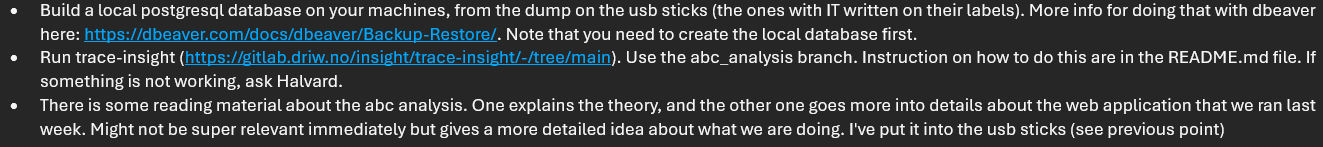
\includegraphics[width=1\linewidth]{ukentlige logger/images/uke 2/email_instructions_week_2.png}
\caption{\label{fig:downloads}E-post med oppgaver som må gjøres.}
\end{figure}

Dette forstatte ut dagen til klokken ble 14:00 da studenten måtte dra for å rekke en forelesing.
}\\\\\\
\logg{Torsdag 19. September}{09:00 til 16:00 (7 timer)}{
Møtte opp klokken 09:00 for å forbrede seg på et møte med \textit{RnD} gruppen som skulle ta sted klokken 10:00. I mellom disse to tidene gjorde studenten seg klar for å fylle ut kontrakt-avtale mellom studenten, universitetet og bedriften. \\

Dette ble fulgt opp av at møtet blir litt forsinket av en gruppemedlem er forsinket for møtet. Møtet startet da derfor 1030. På møtet ble studenten introdusert til den lineære matematikken bak abc-analyse formelen og hvordan denne matematikken blir brukt i bedriften. Her fikk studenten vite om diverse begreper som bedriften bruker; \textit{Activity}, \textit{Item}, \textit{Measure}, og \textit{Cost}. Aktivitet refererer til hvilket stadiet produktet er i. Om den er i transport, ligger i et varehus, eller rett og slett rotner. Produkt refererer til Hvordan produkt som man snakker om. Det kan være både gulrøtter og treverk, som eksempel. Måling er hva man måler absert på hva kost er. Kost kan variere om hva det er. Det kan være hvor mye CO2 utslipp produktet påfører, eller hvor mye penger dette produktet koster å transportere eller lagre. 

\begin{figure}[H]
\centering
\includegraphics[width=0.50\linewidth]{ukentlige logger/images/uke 2/abc_analysis_basics.jpg}
\caption{\label{fig:downloads}Skisse over abc-analyse.}
\end{figure}

Etter møtet begynte studenten å fortsette jobben på databasen og trace-insight applikasjonen fra gårsdagen. Studenten fikk hjelp av en ansatt på bedriften. Det viser seg at trace-insight sin dokumentasjon var skrevet feil, og noe av koden ikke fungerte lenger. Dette gjorde det naturligvis vansklig for studenten å få startet opp applikasjonen. Den ansatte rettet da opp i feilen i koden og dokumentasjonen og \textit{pushet} det til repositoriet slik at studenten kunne \textit{pulle} det. 

Studenten fikk også hjelp til databasen, ettersom når dataen fra dump-filen ble gjennopprettet, ble ikke all dataen det. Noe som gjorde at studenten fikk hjelp til å opprette all dataten. Resultatet er ikke bekreftet ettersom det tar lang tid å opprette denne dataen (ingen vet hvorfor det tar så lang tid). \\

Etter at alle applikasjonene fungerer og databasen jobber med å gjenopprette dataen, begynte studenten og medstudentene å se på matematikken bak abc-analysen, for å kunne få en dypere forsåelse på hvordan den brukes. Dette ble gjort ved å se på diverse caser som kan skje. Her satt studentene og gjorde matte for å forså hvordan formelen fungerer.\\

Etter at studentene kom fram til en stopp, bestemte studenten Vegard Arnesen Mytting å dra hjem. Ettersom klokken var over 16:00. 
}\\\\\\
\logg{Onsdag 25. September}{09:00 til 14:00 (5 timer)}{
Møtte opp klokken 09:00 for å sjekke om all dataen til databasen har blitt gjenopprettet fra uken tidligere. Det har den ikke. Dette kan være på grunn av at laptopen ikke ble brukt. 

Studenten innså også på vei inn på kontoret at det var en monitor med diverse kabler på bordet. Studenten valgte da å koble opp monitoren til laptopen. \\ 

Etter dette bestemte studenten seg for å begynne å \textit{forstå} koden som allerede er bygget på applikasjonen som skal bli skrevet over fra \textit{Python} til \textit{java}, for å få en idé om hvordan applikasjonen vil bli bygget opp. Etter dette begynte studenten å lære seg frontend-rammeverket \textit{Vue3}.\\

klokken 11:00 spurte eleven om hjelp med dataen til databasen. Det ble konkludert med at studenten skal vente å se om dataen kommer etterhvert. Ettersom når laptopen gikk i hvilemodus, stoppet gjenopprettingen prosessen sin. \\

Etter dette møtet med en ansatt på bedriften, fortsatte studenten å lese gjennom og prøve å forstå koden som allerede eksisterer med den teknologien som blir brukt.\\

Da klokken ble 14:00, begynte studenten å pakke sammen sakene sine for å så dra for å rekke en forelesning.
}\\\\\\
\logg{Torsdag 26. September}{09:00 til 12:30 (3,5 timer)}{
Møtte opp klokken 09:00 for å fortsette å lese gjennom koden og forstå hvordan koden er satt opp. Etter litt lesing bestemte studenten seg for å eksperimentere i koden. Studenten lagde så et vindu til hvor den nye modulen av applikasjonen skal være. Dette ble gjort for å kunne forstå hvordan \textit{frontend} kode-stilen og teknologien til bedriften er.\\ 

Etter dette ble oppgaver fordelt på tvers av teamet. Studenten Vegard Arnesen Mytting fikk jobben til å skrive \textit{backend} til applikasjonen. Med andre ord, fikse backend endpointen til \textit{API}'en som skal skrives.\\

\textit{Postman} ble dermed lastet ned for å teste ut den allerede eksisterende backend endpointet. Etter alle testene ble skrevet, begynte studenten å se gjennom backend på python web applikasjonen for å kunne få mer kunnskap om hvordan java web applikasjonen kommer til å se ut.\\

Etter dette begynte studenten å skrive den nye java backend koden med å lage en \textit{model} klasse, en \textit{service} klasse og en \textit{controller} klasse.\\

Når klokken ble 12:30 måtte studenten dra for dagen.
}\\\\\\
\logg{Onsdag 02. Oktober}{10:00 til 14:00 (4 timer)}{
Møtte opp klokken 10:00 i dag. Kom tilbake til kontoret med møtet på at datamaskinen min er død. Dette er et problem ettersom gjenopprettingen av databasen ikke ble fullført. Heldigvis var mye av den relevante dataen gjenopprettet, noe som gjør at studenten bestemte seg for å ikke jobbe mer med det. \\

Dermed bestemte studenten seg for å fortsette å kode matematikken/logikken som skal brukes i applikasjonen. Her lagde studenten noen \textit{Issues} om hva som må bli gjort.

\begin{figure}[H]
\centering
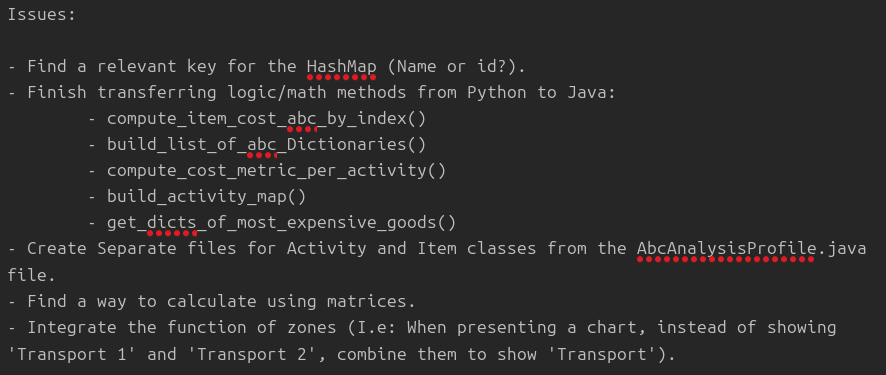
\includegraphics[width=1\linewidth]{ukentlige logger/images/uke 4/issues 02.10.png}
\caption{\label{fig:downloads}Issues fra Onsdag 02. Oktober.}
\end{figure}

Studenten Vegard Arnesen Mytting dro for å rekke en forelesing klokken 14:00.
}\\\\\\
\logg{Torsdag 03. Oktober}{10:00 til 16:00 (6 timer)}{
Måtte opp klokken 10:00 i dag. Begynte å fortsette å jobbe med matten/logikken i backend. \\

Rundt klokken 12:30 hadde gruppen \textit{RnD} et møte for å oppdatere hverandre på hva som er gjort. Her ble en prototype på frontend presentert, hvordan kodestrukturen burde være og hvor langt logikken/matten er kommet. På møtet ble også studentene fortalt at \textit{Andrea Tenti} skal finne noen som kan fortelle oss hva som er relevant data for oss, slik at vi kan begynne å koble oss på databasen. Etter dette fortsatte studentene med arbeidet sitt.\\

Studenten Vegard Arnesen Mytting dra hjem 16:00.
}\\\\\\
\logg{Onsdag 09. Oktober}{08:00 til 14:00 (6 timer)}{
Møtte opp klokken 08:00 i dag. Begynte å jobbe med matten igjen. Denne gangen ble det sett mer på 'zone' attributtet. Denne attributtet sin jobb er å dele alle aktivitene inn i forskjellige soner, dersom det trengs. \\

Det ble jobbet med hele dagen. Ble desverre ikke noe god framgang.
}\\\\\\
\logg{Torsdag 10. Oktober}{09:00 til 16:00 (7 timer)}{
Møtte opp klokken 09:00 for å jobbe med matten, og få mulighet til å spørre Andrea Tenti spørsmål om applikasjonen. Andrea var desverre ikke på kontoret i dag da jeg kom. Så jeg jobbet videre med Zone funksjonen.\\

Når klokken ble 12:00 gikk jeg for å spise lunsj. etter ca. 30 min kom Andrea Tenti for å spise lunsj han også. Etter at alle har spist, stilte jeg han spørsmål om applikasjonen. \\

Han ønsket å \textit{hash'e} verdiene fra databasen, slik at det blir lett å teste funksjonene (slik at det ikke har noe å si dersom man tester med \textit{String} verdier eller \textit{Integer} verdier). \\

Han viste meg også hvordan man skal finne diverse verdier fra databasen. Her innså jeg at databasen var veldig avansert og var derfor komplisert og vanskelig å følge med i gjennomgangen. \\

Jeg begynte derfor å bli stresset over hva som må til, siden jeg hadde ingen anelse om hva som skal gjøres.
}\\\\\\
\logg{Torsdag 17. Oktober}{09:00 til 15:00 (6 timer)}{
Møtte opp klokken 09:00 i dag. Jeg fortsatte med Zone funksjonen.\\

I dag fikk jeg endelig til Zone fuksjonen til å fungere. Alle metodene ble implementert og de fungerer som de skal.\\

Metoder ble laget, men testene måtte vente til morgen dagen. Ettersom da jeg fullførte alle metodene, måtte jeg dra.
}\\\\\\
\logg{Fredag 18. Oktober}{09:30 til 15:00 (5.5 timer)}{
I dag lagde jeg tester for alle metodene mine for å dobbel & trippel sjekke at de fungerer som de skal. \\

Metodene fungerte perfekt, bortsett fra at metodene var avhengig av at det bare var \textit{en} type vare som ble bearbeidet. Dette må endres til at metodene kan bearbeide flere varer samtidig. \\

Dette var en ganske enkel fiks, med å bare legge til en simpel \textit{if-statement} for å filtrere relevante varer til abc-analysen. \\

Etter denne fiksen og testene, måtte jeg dra.
}\\\\\\
\logg{Onsdag 23. Oktober}{08:00 til 16:00 (8 timer)}{
Møtte opp 08:00 i dag. Fortsatte med å kode matematikken, med hoved fokus på å fikse en \textit{controller} klasse for å begynne med \textit{API} testing. Etter at denne metoden ble implementert, skulle jeg begynne å teste. Det var her jeg innså at jeg ikke visste hvordan, fordi jeg har ikke koblet koden opp til databasen. \\

Etter litt diskusjon med gruppemedlem om hva som må gjøres, innså jeg at koden jeg har skrivet ikke er i samme \textit{stil} som selvskapet gjør. Dette gjør at koden min ikke nødvendligvis vil \textit{oppføre} seg riktig med henhold til hvordan alt annet er satt opp. Jeg ble da nødt til å revurdere hvordan jeg skal bygge opp matte-koden jeg hars skrevet. \\

Etter en lunsj-pause skjønte jeg at jeg måtte lage en query som gjør matten i seg. Dette vil føre til at man gjør alle operasjonene \textit{nærme dataen}, noe som er ønsket. Jeg begynte så å se på hvordan selskapet har skrevet querier før, og hvordan deres oppsett vil være. Dette fortsatte jeg med resten av dagen.
}\\\\\\
\logg{Torsdag 24. Oktober}{08:00 til 16:00 (8 timer)}{
Møtte opp 08:00 i dag. hele dagen i dag og slutt-delen av gårsdagen ble brukt for å finne ut av hvordan queryene til selskapet blir laget. \\

Jeg klarte å fullføre en query i dag som returnerer det som er ønsket. Dette gikk fort ettersom jeg har brukt lang tid på å porgrammere hele prosessen, så jeg visste sånn ish hva som måtte bli gjort for å fullføre det. \\

For å kunne teste det ordentlig, lagde jeg noen test \textit{tables} i databasen og fylte dem med verider som jeg visste resultatene til. Etter å ha fått tilfredstillende resulatter, viste jeg koden og database oppsettet til en annen gruppemedlem og vi diskuterte om hva som skal så bli gjort. Vi ble enige at koden og strukturen jeg hadde ga med mening, og var mer optimal. \\

Vi da brukte resten av dagen på å få databasen hans til å ha samma database struktur og begynte å teste API'en med postman.
}\\\\\\
\logg{Fredag 25. Oktober}{08:00 til 16:00 (8 timer)}{
Møtte opp 08:00 i dag. Dagen i dag gikk til å lære seg database oppsattet til selskapet (ikke test \textit{tablesene} som jeg lagde) og frontend strukturen til selskapet. \\

Etter å ha sett på det er par timer lagde jeg en \textit{MVP} for hva oppgaven spurte om, jeg fullførte da hva oppgaven vi hadde var, men det var med test-verdiene. Med abc-analysen viste profilen sin, og det ser jeg på som vellykket!\\

Jeg vet at en annen gruppemedlem har mer oversikt over koden, så jeg skal ikke \textit{pushe} til \textit{GitLab} det jeg har gjort, ettersom han har mer erfaring med frontend strukturen til selskapet enn det jeg har.\\

Med andre ord, i dag har jeg bare sett på strukturen til databasen og frontenden til selskapet.
}\\\\\\
\logg{Mandag 28. Oktober}{08:00 til 12:30 (4,5 timer)}{
Møtte opp klokken 08:00 i dag. Dagen i dag gikk til å se etter måter å ikke ha \textit{randomized} data i applikasjonen. \\

Per nå er dataen som vises, og dataen som presenteres to foskjellige verdier. Dette er det dagen gikk til. \\

Etter lunsjen, dro jeg hjem for å jobbe videre på en obligatorisk oppgave i et annet emne.
}\\\\\\
\logg{Tirsdag 29. Oktober}{08:30 til 12:30 (4 timer)}{
Møtte opp klokken 08:30 i dag. I dag fortsatte jeg arbeidet som jeg etterlot i går. Dette betyr at jeg forsatte med å finne en løsning på 'visnings og kalkulasjons' problemet. \\

Jeg diskuterte problemet med en annen med-student. Vi diskuterte flere problemer vi hadde. Som: 

\begin{itemize}
    \item at kunden skal kunne endre kost når dem vil.
    \item problemet med randomized data.
    \item problemet med visning og kalkulering av forskjellige verdier.
\end{itemize}

Per nå er kosten randomized, uten at den kan bli endret. Med andre ord, så henger mye av disse problemene sammen i hverandre. Vi prøver å unngå å lage en egen database \textit{table}, ettersom vi burde holde strukturen som bedriften allerede har. \\

Problemet ble dessverre ikke løst i dag.
}\\\\\\
\logg{Onsdag 30. Oktober}{08:00 til 16:00 (8 timer)}{
Møtte opp 08:00 i dag. Dagen i dag gikk til å lese meg opp på diverse løsninger for å løse 'visning og kalkulerings problemet'. Her ble det drøftet om å ikke gjøre kalkulasjonene i backend, men i frontend. Dette er noe vi vil unngå, ettersom vi vil holde all bearbeiding av data så nærme databasen som mulig. \\

Dermed fant jeg ut av en SQL funksjon, hvor man kan lage \textit{temporary} database \textit{tables}. Dette ble testet i \textit{DBeaver}-applikasjonen om det i det hele tatt er mulig. Noe som det viser seg, at det er. Midlertidig \textit{tables} virker som at det skal fungere fint. \\

Resten av dagen gikk da til å implementere dette inn i java-applikasjonen ved å bruke bedriften sin kodestil og API-håndterer.
}\\\\\\
\logg{Torsdag 31. Oktober}{08:00 til 16:00 (8 timer)}{
Møtte opp klokken 08:00 i dag. I dag fortsatte jeg med å implementere \textit{temporary tables}. Jeg hadde en hard tid med å implementere dette i bedriftens API-håndterer. \\

Etter en stund med \textit{trial and error}, spurte jeg en ansatt om hjelp. Det viser seg, at API-håntereren IKKE kan gjøre slike queries. Den er nødt til å returnere en \textit{table} av et slag. Noe denne funksjonen ikke gjør. Ettersom jeg vil holde meg til bedriftens kodestil, ønsket jeg ikke å lage en ny API-hånterer bare for å lage en \textit{temporary table}. \\

Resten av dagen gikk da derfor på å finne andre løsninger, og se mer på databasen.
}\\\\\\
\logg{Fredag 01. November}{08:00 til 16:00 (8 timer)}{
Møtte opp klokken 08:00 i dag. Dagen i dag gikk til å fortsette å løse 'visnings og kalkulerings' problemet. \\ 

Etter lang tid med å prøve å lage en \textit{temporary table}, bruke API-håndterere som ikke fungerer med denne type query, og lage egne API-håndterere, endte det opp med å finne noe relevant data i databasen som man kan bruke som \textit{Activity Cost}. \\

Etter å ha funnet noe som kan fungere, begynte jeg å lage en query for dette. Dagen gikk til dette.
}\\\\\\
\logg{Mandag 04. November}{08:30 til 13:30 (5 timer)}{
Møtte opp klokken 08:00 i dag. Dagen i dag gikk for å finpusse applikasjonen.\\

Kosten til aktivitetene endte opp med å bli summen av hver \textit{instance} av aktivitets-typene (\textit{COUNT(*) AS activity\_cost}). \\

Resten av dagen gikk for å oversette appliaksjonen. Lage en norsk og engelsk versjon av \textit{abc-analyse rapporten}.
}\\\\\\
\logg{Torsdag 07. November}{11:30 til 14:00 (2,5 timer)}{
Møtte opp klokken 11:30 til avslutningen av praksistiden til alle praktikantene som Solwr tok inn.\\

Her ble det spist lunsj, alle prosjektene ble visst fram forran alle ansatte, og gaver ble utgitt til praktikantene. \\

RnD gruppa hadde en siste jobb å gjøre før alle var ferdig. Andrea Tenti ønsket en rask dokumentasjon på hvordan applikasjonen fungerer og hva/når API'ene blir kjørt fra frontend. \\

Dette var det siste som ble gjort.
}